%% -----------------------------------
%% Charlie Redmon
%% 20170923
%% SEM path diagram for semPlot output
%% -----------------------------------

% standalone class for individual image to be included in a document
% border=15pt controls the whitespace padding around the diagram
\documentclass[border=15pt]{standalone}
\usepackage{tikz}

% node/path styles

                \tikzstyle{ov}=[shape=rectangle, draw=black!80,
                  minimum height=0.6cm, minimum width=0.6cm, thick]

                \tikzstyle{av}=[shape=rectangle, draw=black!80,
                  fill=black!10, minimum height=0.6cm, minimum width=0.6cm,
                  thick]

                \tikzstyle{lv}=[shape=circle, draw=black!80, minimum width=1cm,
                  thick]

                \tikzstyle{lcor}=[bend left=30, dashed]

                \tikzstyle{rcor}=[bend right=30, dashed]

                \tikzstyle{lloop}=[loop left, out=150, in=210, 
                  distance=0.3cm, densely dotted]

                \tikzstyle{rloop}=[loop right, out=30, in=-30, 
                  distance=0.3cm, densely dotted]
                \tikzstyle{aloop}=[loop above, out=60, in=120, 
                  distance=0.3cm, densely dotted]
                \tikzstyle{bloop}=[loop below, out=-60, in=-120, 
                  distance=0.3cm, densely dotted]


                \begin{document}

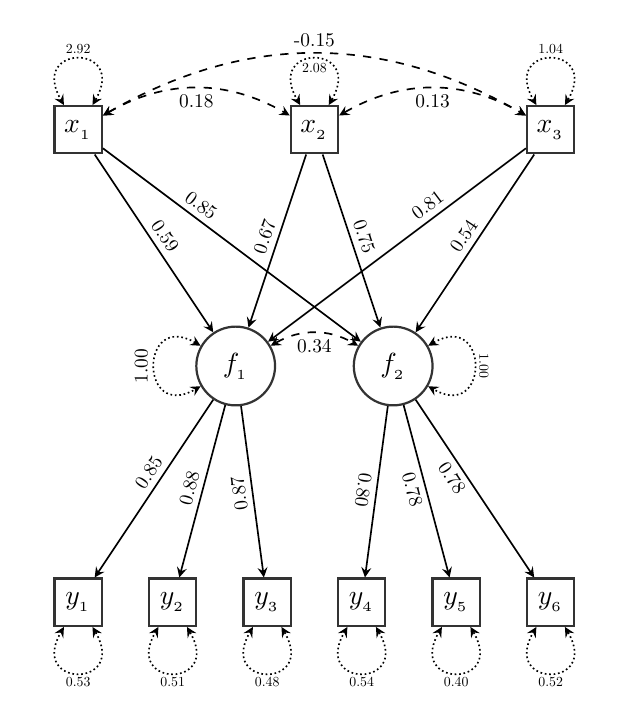
\begin{tikzpicture}[>=stealth, semithick, scale=3]

% nodes
\node[ov] (y1) at (-1,-1) {$y_{_1}$};
\node[ov] (y2) at (-0.6,-1) {$y_{_2}$};
\node[ov] (y3) at (-0.2,-1) {$y_{_3}$};
\node[ov] (y4) at (0.2,-1) {$y_{_4}$};
\node[ov] (y5) at (0.6,-1) {$y_{_5}$};
\node[ov] (y6) at (1,-1) {$y_{_6}$};
\node[ov] (x1) at (-1,1) {$x_{_1}$};
\node[ov] (x2) at (0,1) {$x_{_2}$};
\node[ov] (x3) at (1,1) {$x_{_3}$};
\node[lv] (f1) at (-0.333333333333333,0) {$f_{_1}$};
\node[lv] (f2) at (0.333333333333333,0) {$f_{_2}$};

% paths
\path[->] (f1) edge node[sloped, above, pos=0.45, scale=0.7] {0.85} (y1);
\path[->] (f1) edge node[sloped, above, scale=0.7] {0.88} (y2);
\path[->] (f1) edge node[sloped, above, rotate=180, scale=0.7] {0.87} (y3);
\path[->] (f2) edge node[sloped, below, rotate=180, scale=0.7] {0.80} (y4);
\path[->] (f2) edge node[sloped, below, pos=0.47, scale=0.7] {0.78} (y5);
\path[->] (f2) edge node[sloped, below, pos=0.4, scale=0.7] {0.78} (y6);
\path[->] (x1) edge node[sloped, above, scale=0.7] {0.59} (f1);
\path[->] (x2) edge node[sloped, above, scale=0.7] {0.67} (f1);
\path[->] (x3) edge node[sloped, above, pos=0.35, scale=0.7] {0.81} (f1);
\path[->] (x1) edge node[sloped, above, pos=0.35, scale=0.7] {0.85} (f2);
\path[->] (x2) edge node[sloped, above, scale=0.7] {0.75} (f2);
\path[->] (x3) edge node[sloped, above, scale=0.7] {0.54} (f2);
\path[<->] (y1) edge[bloop] node[sloped, below, scale=0.5] {0.53} (y1);
\path[<->] (y2) edge[bloop] node[sloped, below, scale=0.5] {0.51} (y2);
\path[<->] (y3) edge[bloop] node[sloped, below, scale=0.5] {0.48} (y3);
\path[<->] (y4) edge[bloop] node[sloped, below, scale=0.5] {0.54} (y4);
\path[<->] (y5) edge[bloop] node[sloped, below, scale=0.5] {0.40} (y5);
\path[<->] (y6) edge[bloop] node[sloped, below, scale=0.5] {0.52} (y6);
\path[<->] (f1) edge[lloop] node[sloped, above, rotate=180, scale=0.7] {1.00} (f1);
\path[<->] (f2) edge[rloop] node[sloped, above, scale=0.5] {1.00} (f2);
\path[<->] (f1) edge[lcor] node[sloped, below, scale=0.7] {0.34} (f2);
\path[<->] (x1) edge[aloop] node[sloped, above, scale=0.5] {2.92} (x1);
\path[<->] (x1) edge[lcor] node[sloped, below, scale=0.7] {0.18} (x2);
\path[<->] (x1) edge[lcor] node[sloped, above, scale=0.7] {-0.15} (x3);
\path[<->] (x2) edge[aloop] node[sloped, below, scale=0.5] {2.08} (x2);
\path[<->] (x2) edge[lcor] node[sloped, below, scale=0.7] {0.13} (x3);
\path[<->] (x3) edge[aloop] node[sloped, above, scale=0.5] {1.04} (x3);

\end{tikzpicture}

\end{document}

